\documentclass[14pt,a4paper]{extarticle}
\usepackage[utf8]{inputenc}
\usepackage[T2A]{fontenc}
\usepackage[russian,english]{babel}
\usepackage{mathptmx}
\usepackage[left=25mm, right=15mm, top=20mm, bottom=20mm]{geometry}
\usepackage{graphicx}
\graphicspath{{../img/}}
\usepackage{float}
\usepackage{booktabs}
\usepackage{longtable}
\usepackage{array}
\usepackage{tabularx}
\usepackage{multirow}
\usepackage{minted}
\usepackage{xcolor}
\setminted[sql]{
  frame=single,
  fontsize=\small,
  breaklines=true,
  breakanywhere=true,
  tabsize=4,
  bgcolor=gray!5
}
\usepackage{hyperref}
\hypersetup{
  colorlinks=true,
  linkcolor=black,
  urlcolor=blue
}
\usepackage{setspace}
\usepackage{parskip}
\usepackage{fancyhdr}
\usepackage{titlesec}
\usepackage{caption}
\pagestyle{fancy}
\fancyhf{}
\fancyfoot[C]{\thepage}
\renewcommand{\headrulewidth}{0pt}
\titleformat{\section}{\large\bfseries}{\thesection.}{0.5em}{}
\titleformat{\subsection}{\normalsize\bfseries}{\thesubsection.}{0.5em}{}

\begin{document}

%  ТИТУЛЬНЫЙ ЛИСТ
\begin{titlepage}
  \begin{center}
    \textbf{Министерство науки и высшего образования Российской Федерации}\\[0.3cm]
    \textbf{Федеральное государственное автономное образовательное учреждение\\
    высшего образования}\\[0.3cm]
    \textbf{«НАЦИОНАЛЬНЫЙ ИССЛЕДОВАТЕЛЬСКИЙ УНИВЕРСИТЕТ ИТМО»}\\[2cm]

    \textbf{\Large Хранение и обработка данных}\\[0.5cm]
    \textbf{\large Итоговый проект}\\[1cm]

    \rule{\linewidth}{0.5pt}\\[0.3cm]
    \textbf{\LARGE Спортивный турнир}\\[0.2cm]
    \textbf{\large Матчи Бундеслиги (Германия), сезоны 2020--2023}\\[0.2cm]
    \textbf{Тема 12}\\[0.3cm]
    \rule{\linewidth}{0.5pt}\\[2cm]

    \begin{flushleft}
      \hspace{7cm}
      \begin{minipage}{8cm}
        \textbf{Выполнил:}\\
        \textbf{Ануфриев Андрей Сергеевич}\\[0.3cm]
        \textbf{Группа:} \textbf{R3136}\\[0.3cm]
        \textbf{Номер ИСУ:} 465029\\[0.3cm]
        \textbf{Схема БД:} bk\_465029\_2026\\[0.3cm]

      \end{minipage}
    \end{flushleft}

    \vfill
    \textbf{Санкт-Петербург, 2026}
  \end{center}
\end{titlepage}

%  СОДЕРЖАНИЕ
\tableofcontents
\newpage

\section{Описание предметной области}

\subsection{Общая характеристика}

Предметная область данного проекта — \textbf{профессиональный футбольный турнир}.
В качестве конкретного примера выбрана \textbf{Бундеслига} (Германия) — первая по
значимости футбольная лига Германии, входящая в пятёрку ведущих европейских
чемпионатов. Период охвата: сезоны \textbf{2020/21, 2021/22, 2022/23 и 2023/24}
(в базе данных обозначены как 2020, 2021, 2022, 2023).

\subsection{Источник данных}

Данные получены через открытый API \textbf{OpenLigaDB}
(\url{https://www.openligadb.de/}) и распространяются по лицензии
\textbf{CC BY} (Creative Commons Attribution). API предоставляет сведения
о матчах, командах, результатах и расписании в формате JSON.

\subsection{Ключевые сущности}

В рамках предметной области выделены следующие сущности:

\begin{itemize}
  \item \textbf{Команда} — клуб-участник Бундеслиги: название, город,
        год основания, домашний стадион, главный тренер.
  \item \textbf{Стадион (Venue)} — спортивный объект: название, город, страна,
        вместимость, тип покрытия.
  \item \textbf{Тренер (Coach)} — главный тренер команды: имя, фамилия,
        гражданство, дата рождения.
  \item \textbf{Игрок (Player)} — футболист: имя, фамилия, позиция,
        номер, гражданство, дата рождения.
  \item \textbf{Судья (Referee)} — арбитр матча: имя, фамилия,
        гражданство, категория (FIFA / national).
  \item \textbf{Матч (Match)} — игра: сезон, игровой тур, дата, время,
        команды, стадион, статус (сыгран / отменён).
  \item \textbf{Результат матча (Match Result)} — итог матча: голы хозяев
        и гостей (полное время и первый тайм), победитель.
  \item \textbf{Судейская бригада (Match Referees)} — связь матча с
        судьями и их ролями (главный, ассистент, видеоарбитр).
\end{itemize}

\subsection{Масштаб данных}

База данных содержит \textbf{более 3\,000 записей} в 8 таблицах:
21 команда, 17 стадионов, 21 тренер, 313 игроков, 24 арбитра,
1\,087 матчей с результатами и 523 записи о судейских бригадах.

\section{Описание задач для 10 запросов}

В рамках проекта сформулированы следующие аналитические задачи:

\begin{enumerate}

  \item \textbf{Расписание турнира.}
  Задача: определить, когда, где и с кем играет каждая команда в выбранном
  сезоне. Запрос формирует полное расписание матчей с указанием тура, даты,
  времени, названий команд-участниц, стадиона и города проведения.

  \item \textbf{Итоговая турнирная таблица.}
  Задача: построить классическую турнирную таблицу по итогам сезона. Для каждой
  команды рассчитываются: количество матчей, побед, ничьих и поражений, голы
  забитые и пропущенные, разница голов и итоговые очки (победа~=~3~очка,
  ничья~=~1). Команды сортируются по очкам.

  \item \textbf{Результаты всех матчей с полным счётом и счётом первого тайма.}
  Задача: получить полную таблицу результатов всех сыгранных матчей. Для каждой
  игры отображается счёт по итогам полного времени и по итогам первого тайма,
  а также определяется победитель.

  \item \textbf{Статистика матчей по стадионам.}
  Задача: оценить «результативность» каждого стадиона — среднее и максимальное
  количество голов за матч, а также общее число матчей, проведённых на арене.

  \item \textbf{Команды с наибольшей долей побед на домашнем поле.}
  Задача: проанализировать выступление команд дома — подсчитать количество и
  процент побед, ничьих и поражений в домашних матчах. Выявить команды с
  наиболее высоким процентом домашних побед.

  \item \textbf{Топ-20 результативных матчей.}
  Задача: найти матчи с наибольшим суммарным количеством голов. Вывести
  топ-20 самых результативных игр с указанием счёта, сезона, стадиона.

  \item \textbf{Нагрузка на судей.}
  Задача: определить, сколько матчей обслужил каждый арбитр в разных ролях
  (главный судья, ассистент, видеоарбитр). Выявить наиболее востребованных
  судей за весь рассматриваемый период.

  \item \textbf{Сводная карточка клуба (состав, тренер, стадион).}
  Задача: сформировать справочную карточку каждого клуба — название, город,
  год основания, главный тренер, домашний стадион с вместимостью и число
  игроков в заявке.

  \item \textbf{Среднее количество голов по сезонам и игровым турам.}
  Задача: проследить динамику результативности матчей по сезонам и турам.
  Для каждого тура внутри каждого сезона рассчитывается среднее число голов
  за матч и суммарное число голов, а также распределение исходов
  (победа хозяев, гостей, ничья).

  \item \textbf{Прямые очные встречи двух команд (H2H: Bayern vs Dortmund).}
  Задача: получить историю личных встреч между Bayern München и
  Borussia Dortmund за все рассматриваемые сезоны. Для каждого матча
  указывается дата, счёт и победитель.

\end{enumerate}

\section{ER-диаграмма и описание таблиц}

\subsection{ER-диаграмма}

На рисунке~\ref{fig:er} представлена ER-диаграмма базы данных схемы
\texttt{bk\_465029\_2026}.

\begin{figure}[H]
  \centering
  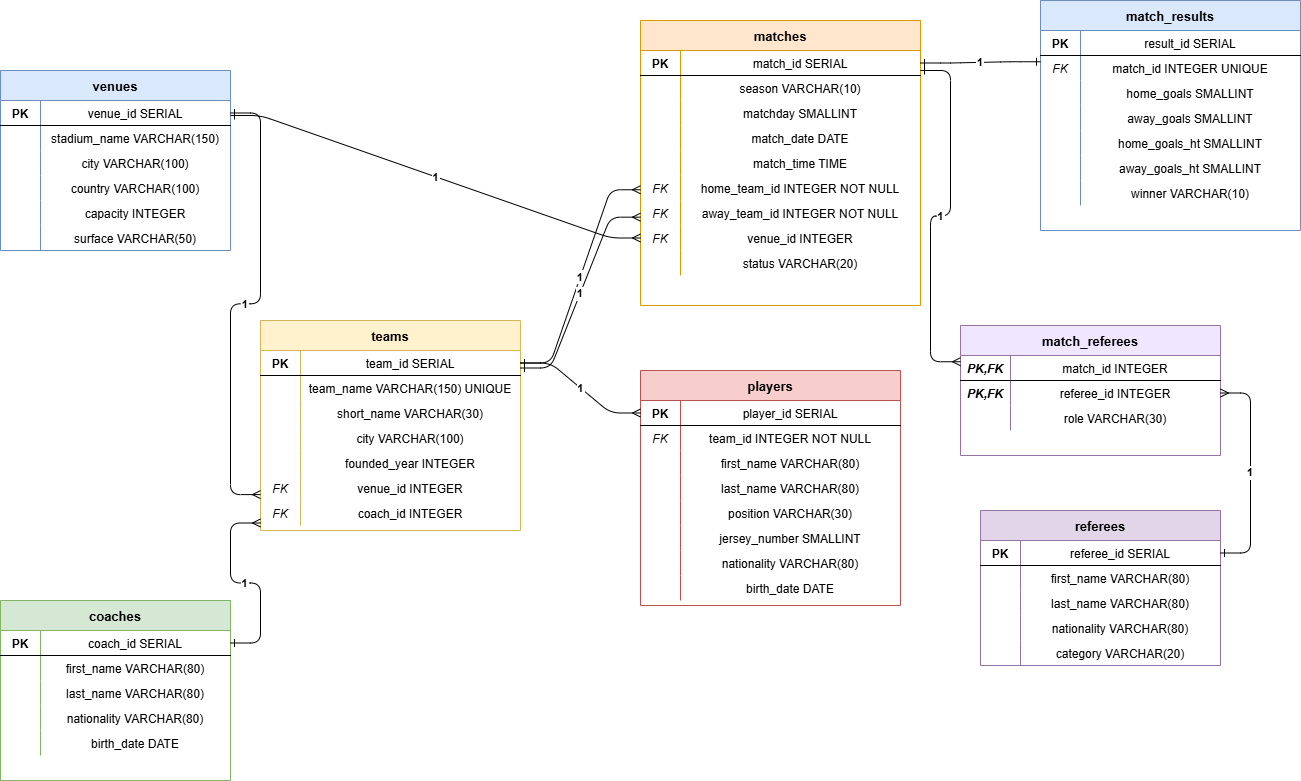
\includegraphics[width=\textwidth]{stage04_er_diagram.png}
  \caption{ER-диаграмма базы данных «Спортивный турнир» (Бундеслига)}
  \label{fig:er}
\end{figure}

\subsection{Описание таблиц}

\begin{longtable}{|p{3.5cm}|p{3.5cm}|p{2cm}|p{5.5cm}|}
  \caption{Таблицы базы данных \texttt{bk\_465029\_2026}}
  \label{tab:tables}\\
  \hline
  \textbf{Таблица} & \textbf{Ключевые столбцы} & \textbf{Строк} & \textbf{Описание} \\
  \hline
  \endfirsthead
  \hline
  \textbf{Таблица} & \textbf{Ключевые столбцы} & \textbf{Строк} & \textbf{Описание} \\
  \hline
  \endhead
  \hline
  \endfoot

  \texttt{venues} &
  venue\_id (PK), stadium\_name, city, country, capacity, surface &
  17 &
  Стадионы: название, город, страна, вместимость, тип покрытия \\
  \hline

  \texttt{coaches} &
  coach\_id (PK), first\_name, last\_name, nationality, birth\_date &
  21 &
  Тренеры команд: ФИО, гражданство, дата рождения \\
  \hline

  \texttt{teams} &
  team\_id (PK), team\_name, short\_name, city, founded\_year, venue\_id (FK), coach\_id (FK) &
  21 &
  Клубы-участники: название, короткое имя, город, год основания, ссылки на стадион и тренера \\
  \hline

  \texttt{players} &
  player\_id (PK), team\_id (FK), first\_name, last\_name, position, jersey\_number, nationality, birth\_date &
  313 &
  Игроки: ФИО, позиция, номер, гражданство, дата рождения \\
  \hline

  \texttt{referees} &
  referee\_id (PK), first\_name, last\_name, nationality, category &
  24 &
  Судьи: ФИО, гражданство, категория (FIFA / national) \\
  \hline

  \texttt{matches} &
  match\_id (PK), season, matchday, match\_date, match\_time, home\_team\_id (FK), away\_team\_id (FK), venue\_id (FK), status &
  1087 &
  Матчи: сезон, тур, дата, время, участники, стадион, статус \\
  \hline

  \texttt{match\_results} &
  result\_id (PK), match\_id (FK), home\_goals, away\_goals, home\_goals\_ht, away\_goals\_ht, winner &
  1087 &
  Результаты матчей: голы хозяев/гостей (полное время и 1-й тайм), победитель \\
  \hline

  \texttt{match\_referees} &
  match\_id (FK), referee\_id (FK), role &
  523 &
  Судейские бригады: связь матча с арбитрами и их ролями \\
  \hline

\end{longtable}

\subsection{Схема связей}

\begin{itemize}
  \item \texttt{teams.venue\_id} $\rightarrow$ \texttt{venues.venue\_id}
  \item \texttt{teams.coach\_id} $\rightarrow$ \texttt{coaches.coach\_id}
  \item \texttt{players.team\_id} $\rightarrow$ \texttt{teams.team\_id}
  \item \texttt{matches.home\_team\_id}, \texttt{matches.away\_team\_id} $\rightarrow$ \texttt{teams.team\_id}
  \item \texttt{matches.venue\_id} $\rightarrow$ \texttt{venues.venue\_id}
  \item \texttt{match\_results.match\_id} $\rightarrow$ \texttt{matches.match\_id}
  \item \texttt{match\_referees.match\_id} $\rightarrow$ \texttt{matches.match\_id}
  \item \texttt{match\_referees.referee\_id} $\rightarrow$ \texttt{referees.referee\_id}
\end{itemize}

\section{Примеры выполнения запросов}

Все запросы выполняются в контексте схемы \texttt{bk\_465029\_2026} базы данных
PostgreSQL PRO. В начале каждой сессии выполняется:
\begin{minted}{sql}
SET search_path TO bk_465029_2026;
\end{minted}

% ----------------------------------------------------------
\subsection{Запрос 1. Расписание турнира}
% ----------------------------------------------------------

\textbf{Задача:} вывести расписание матчей выбранного сезона — дату, время,
команды-участницы, стадион и статус каждого матча.

\begin{listing}[H]
\caption{Расписание турнира (сезон 2023)}
\begin{minted}{sql}
SELECT
    m.season                             AS "Сезон",
    m.matchday                           AS "Тур",
    m.match_date                         AS "Дата",
    m.match_time                         AS "Время",
    ht.team_name                         AS "Хозяева",
    at.team_name                         AS "Гости",
    v.stadium_name                       AS "Стадион",
    v.city                               AS "Город",
    m.status                             AS "Статус"
FROM   matches      m
JOIN   teams        ht ON m.home_team_id = ht.team_id
JOIN   teams        at ON m.away_team_id = at.team_id
LEFT JOIN venues    v  ON m.venue_id     = v.venue_id
WHERE  m.season = '2023'
ORDER BY m.matchday, m.match_date;
\end{minted}
\end{listing}

% ----------------------------------------------------------
\subsection{Запрос 2. Итоговая турнирная таблица}
% ----------------------------------------------------------

\textbf{Задача:} построить турнирную таблицу — очки, победы, ничьи, поражения,
разница голов для каждой команды в выбранном сезоне.

\begin{listing}[H]
\caption{Итоговая турнирная таблица (сезон 2023)}
\begin{minted}{sql}
WITH team_stats AS (
    SELECT
        t.team_name,
        COUNT(*) FILTER (WHERE mr.winner = 'home' AND m.home_team_id = t.team_id
                           OR   mr.winner = 'away' AND m.away_team_id = t.team_id)  AS wins,
        COUNT(*) FILTER (WHERE mr.winner = 'draw')                                   AS draws,
        COUNT(*) FILTER (WHERE mr.winner = 'away' AND m.home_team_id = t.team_id
                           OR   mr.winner = 'home' AND m.away_team_id = t.team_id)  AS losses,
        SUM(CASE WHEN m.home_team_id = t.team_id THEN mr.home_goals
                 ELSE mr.away_goals END)                                              AS goals_for,
        SUM(CASE WHEN m.home_team_id = t.team_id THEN mr.away_goals
                 ELSE mr.home_goals END)                                              AS goals_against
    FROM   teams   t
    JOIN   matches m  ON t.team_id = m.home_team_id
                      OR t.team_id = m.away_team_id
    JOIN   match_results mr ON m.match_id = mr.match_id
    WHERE  m.season = '2023'
    GROUP BY t.team_name
)
SELECT
    ROW_NUMBER() OVER (ORDER BY wins*3 + draws DESC,
                                goals_for - goals_against DESC,
                                goals_for DESC)          AS "Место",
    team_name                                            AS "Команда",
    wins + draws + losses                                AS "И",
    wins                                                 AS "В",
    draws                                                AS "Н",
    losses                                               AS "П",
    goals_for                                            AS "ГЗ",
    goals_against                                        AS "ГП",
    goals_for - goals_against                            AS "РГ",
    wins * 3 + draws                                     AS "Очки"
FROM   team_stats
ORDER BY "Очки" DESC, "РГ" DESC, "ГЗ" DESC;
\end{minted}
\end{listing}

% ----------------------------------------------------------
\subsection{Запрос 3. Результаты всех матчей с полным счётом}
% ----------------------------------------------------------

\textbf{Задача:} получить результаты всех сыгранных матчей с указанием счёта
по полному времени, счёта первого тайма и победителя.

\begin{listing}[H]
\caption{Результаты матчей с полным счётом и счётом первого тайма}
\begin{minted}{sql}
SELECT
    m.season                                      AS "Сезон",
    m.matchday                                    AS "Тур",
    m.match_date                                  AS "Дата",
    ht.team_name                                  AS "Хозяева",
    CONCAT(mr.home_goals, ' : ', mr.away_goals)   AS "Счёт",
    CONCAT(mr.home_goals_ht,' : ',mr.away_goals_ht) AS "Счёт (1 тайм)",
    at.team_name                                  AS "Гости",
    CASE mr.winner
        WHEN 'home' THEN ht.team_name
        WHEN 'away' THEN at.team_name
        ELSE 'Ничья'
    END                                           AS "Победитель"
FROM   matches       m
JOIN   teams         ht ON m.home_team_id = ht.team_id
JOIN   teams         at ON m.away_team_id = at.team_id
JOIN   match_results mr ON m.match_id     = mr.match_id
ORDER  BY m.match_date, m.matchday;
\end{minted}
\end{listing}

% ----------------------------------------------------------
\subsection{Запрос 4. Статистика матчей по стадионам}
% ----------------------------------------------------------

\textbf{Задача:} проанализировать результативность на каждом стадионе —
количество проведённых матчей, среднее и максимальное число голов.

\begin{listing}[H]
\caption{Статистика матчей по стадионам}
\begin{minted}{sql}
SELECT
    v.stadium_name                                AS "Стадион",
    v.city                                        AS "Город",
    v.capacity                                    AS "Вместимость",
    COUNT(m.match_id)                             AS "Матчей сыграно",
    ROUND(AVG(mr.home_goals + mr.away_goals), 2)  AS "Ср. голов/матч",
    MAX(mr.home_goals + mr.away_goals)            AS "Макс голов"
FROM   venues        v
JOIN   matches       m  ON v.venue_id  = m.venue_id
JOIN   match_results mr ON m.match_id  = mr.match_id
GROUP  BY v.venue_id, v.stadium_name, v.city, v.capacity
HAVING COUNT(m.match_id) > 0
ORDER  BY COUNT(m.match_id) DESC;
\end{minted}
\end{listing}

% ----------------------------------------------------------
\subsection{Запрос 5. Команды с наибольшей долей побед дома}
% ----------------------------------------------------------

\textbf{Задача:} рассчитать процент домашних побед для каждой команды и
выявить лидеров по выступлению на родном поле.

\begin{listing}[H]
\caption{Доля домашних побед по командам}
\begin{minted}{sql}
SELECT
    ht.team_name                                        AS "Команда",
    COUNT(*)                                            AS "Домашних матчей",
    COUNT(*) FILTER (WHERE mr.winner = 'home')          AS "Побед дома",
    COUNT(*) FILTER (WHERE mr.winner = 'draw')          AS "Ничьих дома",
    COUNT(*) FILTER (WHERE mr.winner = 'away')          AS "Поражений дома",
    ROUND(100.0 * COUNT(*) FILTER (WHERE mr.winner = 'home')
          / COUNT(*), 1)                                AS "% побед дома"
FROM   matches       m
JOIN   teams         ht ON m.home_team_id = ht.team_id
JOIN   match_results mr ON m.match_id     = mr.match_id
GROUP  BY ht.team_name
ORDER  BY "% побед дома" DESC;
\end{minted}
\end{listing}

% ----------------------------------------------------------
\subsection{Запрос 6. Топ-20 результативных матчей}
% ----------------------------------------------------------

\textbf{Задача:} найти 20 матчей с наибольшим суммарным числом забитых голов.

\begin{listing}[H]
\caption{Топ-20 матчей по количеству голов}
\begin{minted}{sql}
SELECT
    m.season                                      AS "Сезон",
    m.matchday                                    AS "Тур",
    m.match_date                                  AS "Дата",
    ht.team_name                                  AS "Хозяева",
    CONCAT(mr.home_goals,' : ',mr.away_goals)     AS "Счёт",
    at.team_name                                  AS "Гости",
    mr.home_goals + mr.away_goals                 AS "Всего голов",
    v.stadium_name                                AS "Стадион"
FROM   matches       m
JOIN   teams         ht ON m.home_team_id = ht.team_id
JOIN   teams         at ON m.away_team_id = at.team_id
JOIN   match_results mr ON m.match_id     = mr.match_id
LEFT JOIN venues     v  ON m.venue_id     = v.venue_id
ORDER  BY mr.home_goals + mr.away_goals DESC
LIMIT  20;
\end{minted}
\end{listing}

% ----------------------------------------------------------
\subsection{Запрос 7. Нагрузка на судей}
% ----------------------------------------------------------

\textbf{Задача:} подсчитать количество матчей, обслуженных каждым судьёй,
с разбивкой по роли (главный судья / ассистент).

\begin{listing}[H]
\caption{Нагрузка на судей — количество обслуженных матчей}
\begin{minted}{sql}
SELECT
    r.last_name || ' ' || r.first_name            AS "Судья",
    r.nationality                                 AS "Национальность",
    r.category                                    AS "Категория",
    COUNT(*) FILTER (WHERE mref.role = 'main')    AS "Гл. судья",
    COUNT(*) FILTER (WHERE mref.role LIKE 'assistant%') AS "Ассистент",
    COUNT(*)                                      AS "Всего матчей"
FROM   referees      r
JOIN   match_referees mref ON r.referee_id = mref.referee_id
GROUP  BY r.referee_id, r.first_name, r.last_name, r.nationality, r.category
ORDER  BY "Всего матчей" DESC;
\end{minted}
\end{listing}

% ----------------------------------------------------------
\subsection{Запрос 8. Сводная карточка клуба}
% ----------------------------------------------------------

\textbf{Задача:} сформировать информационную карточку каждого клуба —
тренер, домашний стадион и количество игроков в заявке.

\begin{listing}[H]
\caption{Состав команд с тренерами и стадионами}
\begin{minted}{sql}
SELECT
    t.team_name                                   AS "Команда",
    t.city                                        AS "Город",
    t.founded_year                                AS "Год основания",
    c.first_name || ' ' || c.last_name            AS "Тренер",
    c.nationality                                 AS "Нац. тренера",
    v.stadium_name                                AS "Стадион",
    v.capacity                                    AS "Вместимость",
    COUNT(p.player_id)                            AS "Игроков в составе"
FROM   teams   t
LEFT JOIN coaches c ON t.coach_id  = c.coach_id
LEFT JOIN venues  v ON t.venue_id  = v.venue_id
LEFT JOIN players p ON t.team_id   = p.team_id
GROUP  BY t.team_id, t.team_name, t.city, t.founded_year,
          c.first_name, c.last_name, c.nationality,
          v.stadium_name, v.capacity
ORDER  BY t.team_name;
\end{minted}
\end{listing}

% ----------------------------------------------------------
\subsection{Запрос 9. Среднее количество голов по сезонам и турам}
% ----------------------------------------------------------

\textbf{Задача:} проследить динамику результативности по сезонам и игровым
турам — среднее число голов за матч и распределение исходов.

\begin{listing}[H]
\caption{Среднее число голов по сезонам и турам}
\begin{minted}{sql}
SELECT
    m.season                                                   AS "Сезон",
    m.matchday                                                 AS "Тур",
    COUNT(*)                                                   AS "Матчей",
    ROUND(AVG(mr.home_goals + mr.away_goals), 2)               AS "Ср. голов/матч",
    SUM(mr.home_goals + mr.away_goals)                         AS "Всего голов",
    COUNT(*) FILTER (WHERE mr.winner = 'home')                 AS "Побед хозяев",
    COUNT(*) FILTER (WHERE mr.winner = 'away')                 AS "Побед гостей",
    COUNT(*) FILTER (WHERE mr.winner = 'draw')                 AS "Ничьих"
FROM   matches       m
JOIN   match_results mr ON m.match_id = mr.match_id
GROUP  BY m.season, m.matchday
ORDER  BY m.season, m.matchday;
\end{minted}
\end{listing}

% ----------------------------------------------------------
\subsection{Запрос 10. Прямые очные встречи (H2H): Bayern vs Dortmund}
% ----------------------------------------------------------

\textbf{Задача:} получить историю личных встреч между Bayern München и
Borussia Dortmund за все сезоны базы данных.

\begin{listing}[H]
\caption{Личные встречи Bayern München vs Borussia Dortmund (H2H)}
\begin{minted}{sql}
SELECT
    m.season                                      AS "Сезон",
    m.match_date                                  AS "Дата",
    ht.team_name                                  AS "Хозяева",
    CONCAT(mr.home_goals,' : ',mr.away_goals)     AS "Счёт",
    at.team_name                                  AS "Гости",
    CASE mr.winner
        WHEN 'home' THEN ht.team_name || ' победили'
        WHEN 'away' THEN at.team_name || ' победили'
        ELSE 'Ничья'
    END                                           AS "Итог"
FROM   matches       m
JOIN   teams         ht ON m.home_team_id = ht.team_id
JOIN   teams         at ON m.away_team_id = at.team_id
JOIN   match_results mr ON m.match_id     = mr.match_id
WHERE  (ht.team_name = 'Bayern München' AND at.team_name = 'Borussia Dortmund')
    OR (ht.team_name = 'Borussia Dortmund' AND at.team_name = 'Bayern München')
ORDER  BY m.match_date;
\end{minted}
\end{listing}

\section{Примеры визуализации}

В рамках этапа 8 проекта были подготовлены пять визуализаций с использованием
библиотек Python (\texttt{matplotlib}, \texttt{seaborn}, \texttt{pandas}).
Данные для графиков получены из PostgreSQL через SQL-запросы, описанные в
предыдущем разделе.

% ----------------------------------------------------------
\subsection{График 1. Турнирная таблица сезона 2023/24}
% ----------------------------------------------------------

\textbf{Тип:} горизонтальная гистограмма.\\
\textbf{Данные:} итоговые очки команд в сезоне 2023/24, полученные из запроса~2.\\
\textbf{Цель:} наглядно показать расстановку сил в лиге по итогам сезона.

\begin{figure}[H]
  \centering
  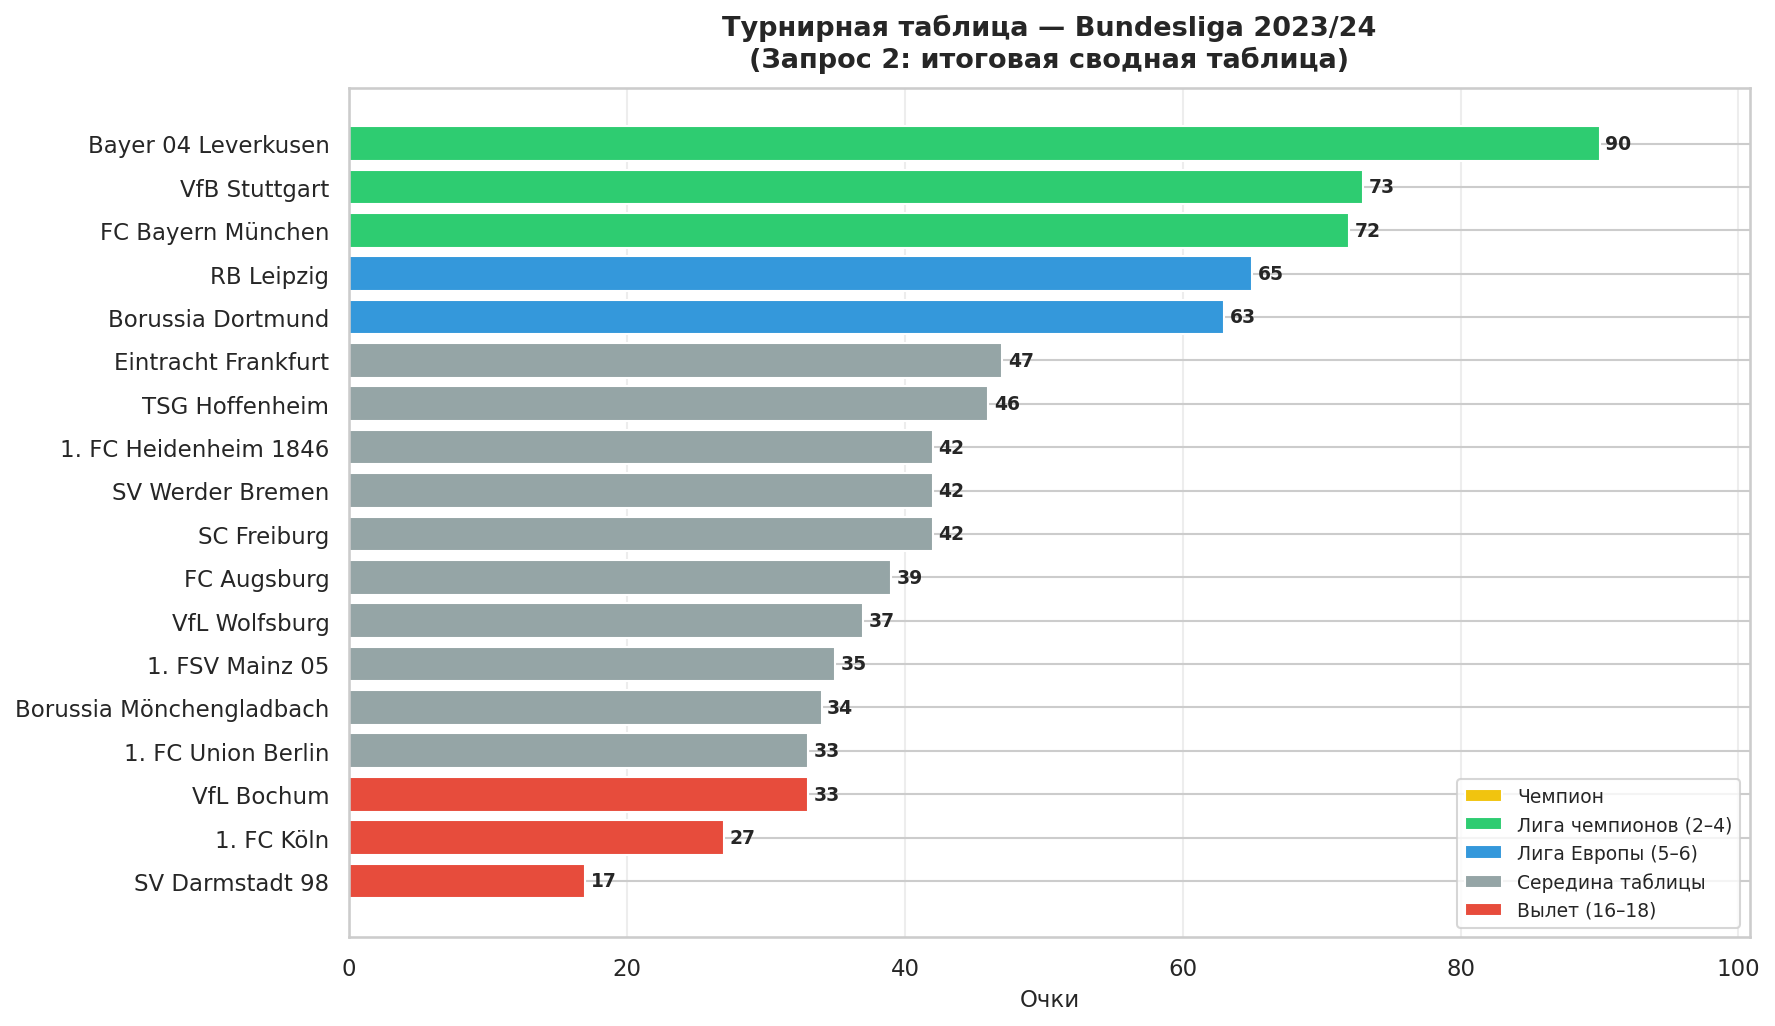
\includegraphics[width=0.85\textwidth]{stage08_viz1_standings.png}
  \caption{Турнирная таблица Бундеслиги, сезон 2023/24 (очки команд)}
  \label{fig:viz1}
\end{figure}

% ----------------------------------------------------------
\subsection{График 2. Среднее забитых голов по командам}
% ----------------------------------------------------------

\textbf{Тип:} горизонтальная гистограмма.\\
\textbf{Данные:} среднее число голов за матч на каждом стадионе (запрос~4).\\
\textbf{Цель:} выявить наиболее результативные арены Бундеслиги.

\begin{figure}[H]
  \centering
  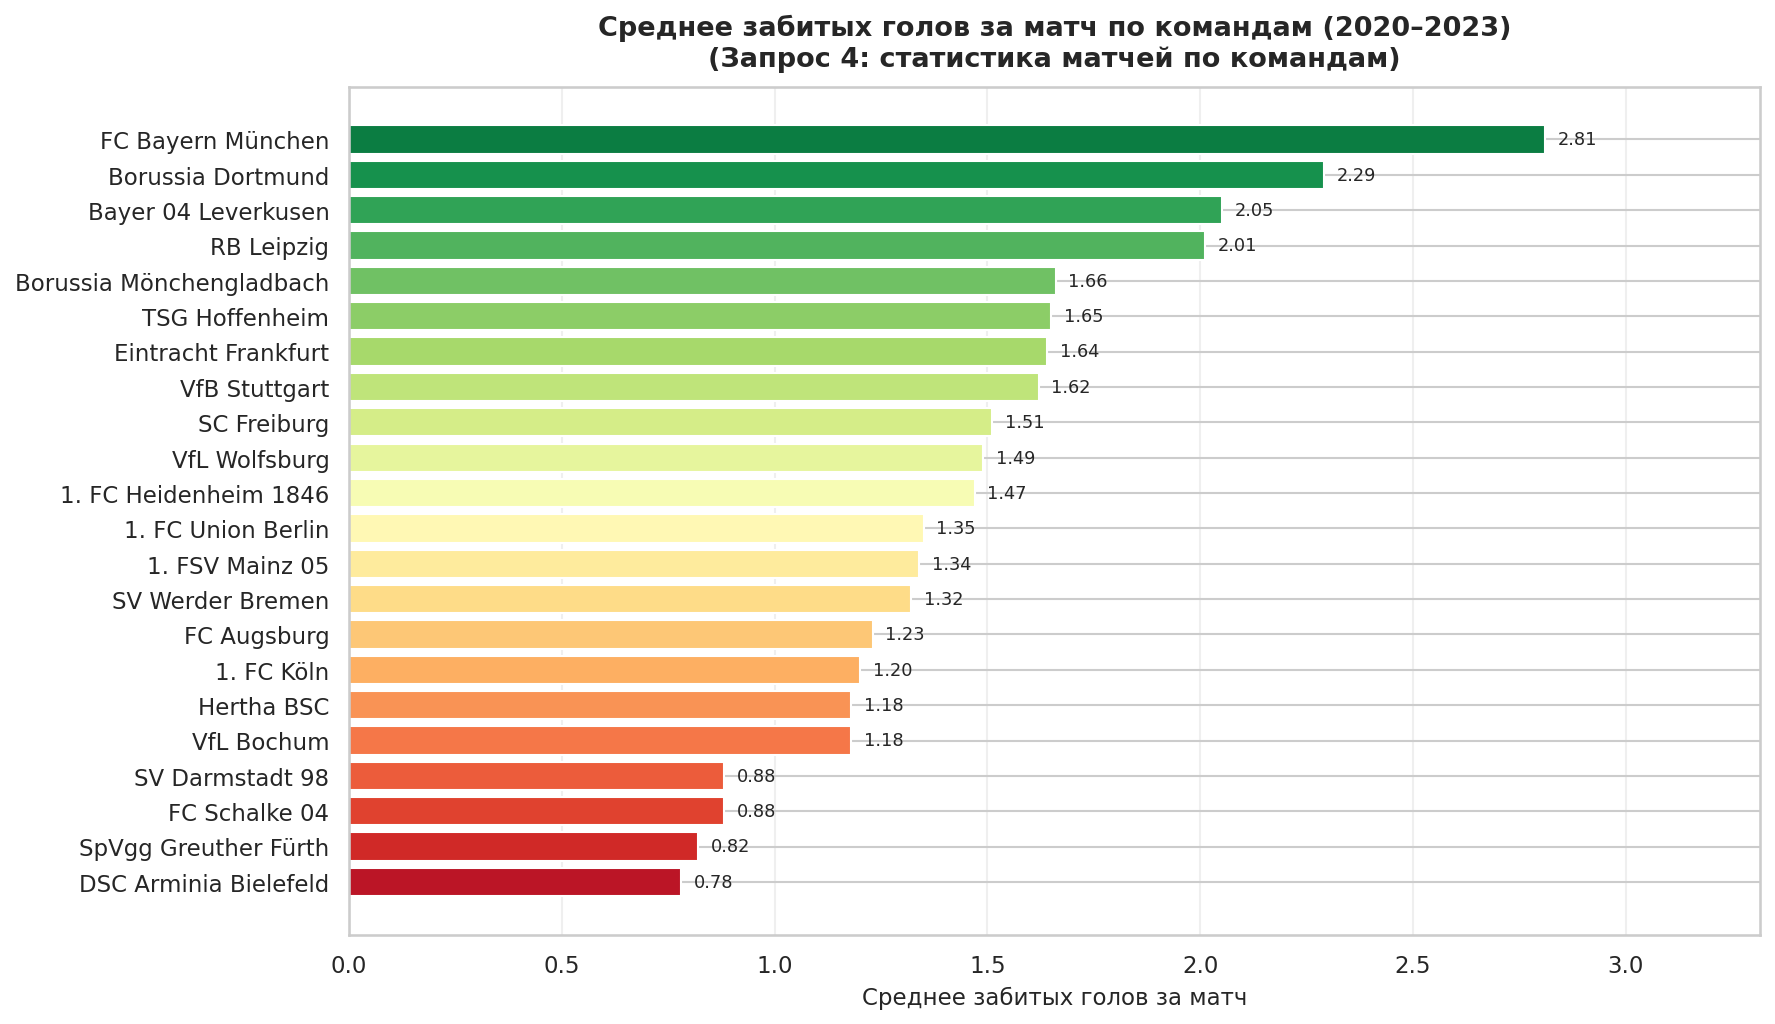
\includegraphics[width=0.85\textwidth]{stage08_viz2_team_goals.png}
  \caption{Среднее количество голов за матч по стадионам}
  \label{fig:viz2}
\end{figure}

% ----------------------------------------------------------
\subsection{График 3. Домашняя статистика команд}
% ----------------------------------------------------------

\textbf{Тип:} составная (stacked) гистограмма.\\
\textbf{Данные:} количество домашних побед, ничьих и поражений для каждой
команды (запрос~5).\\
\textbf{Цель:} сравнить домашние выступления клубов Бундеслиги.

\begin{figure}[H]
  \centering
  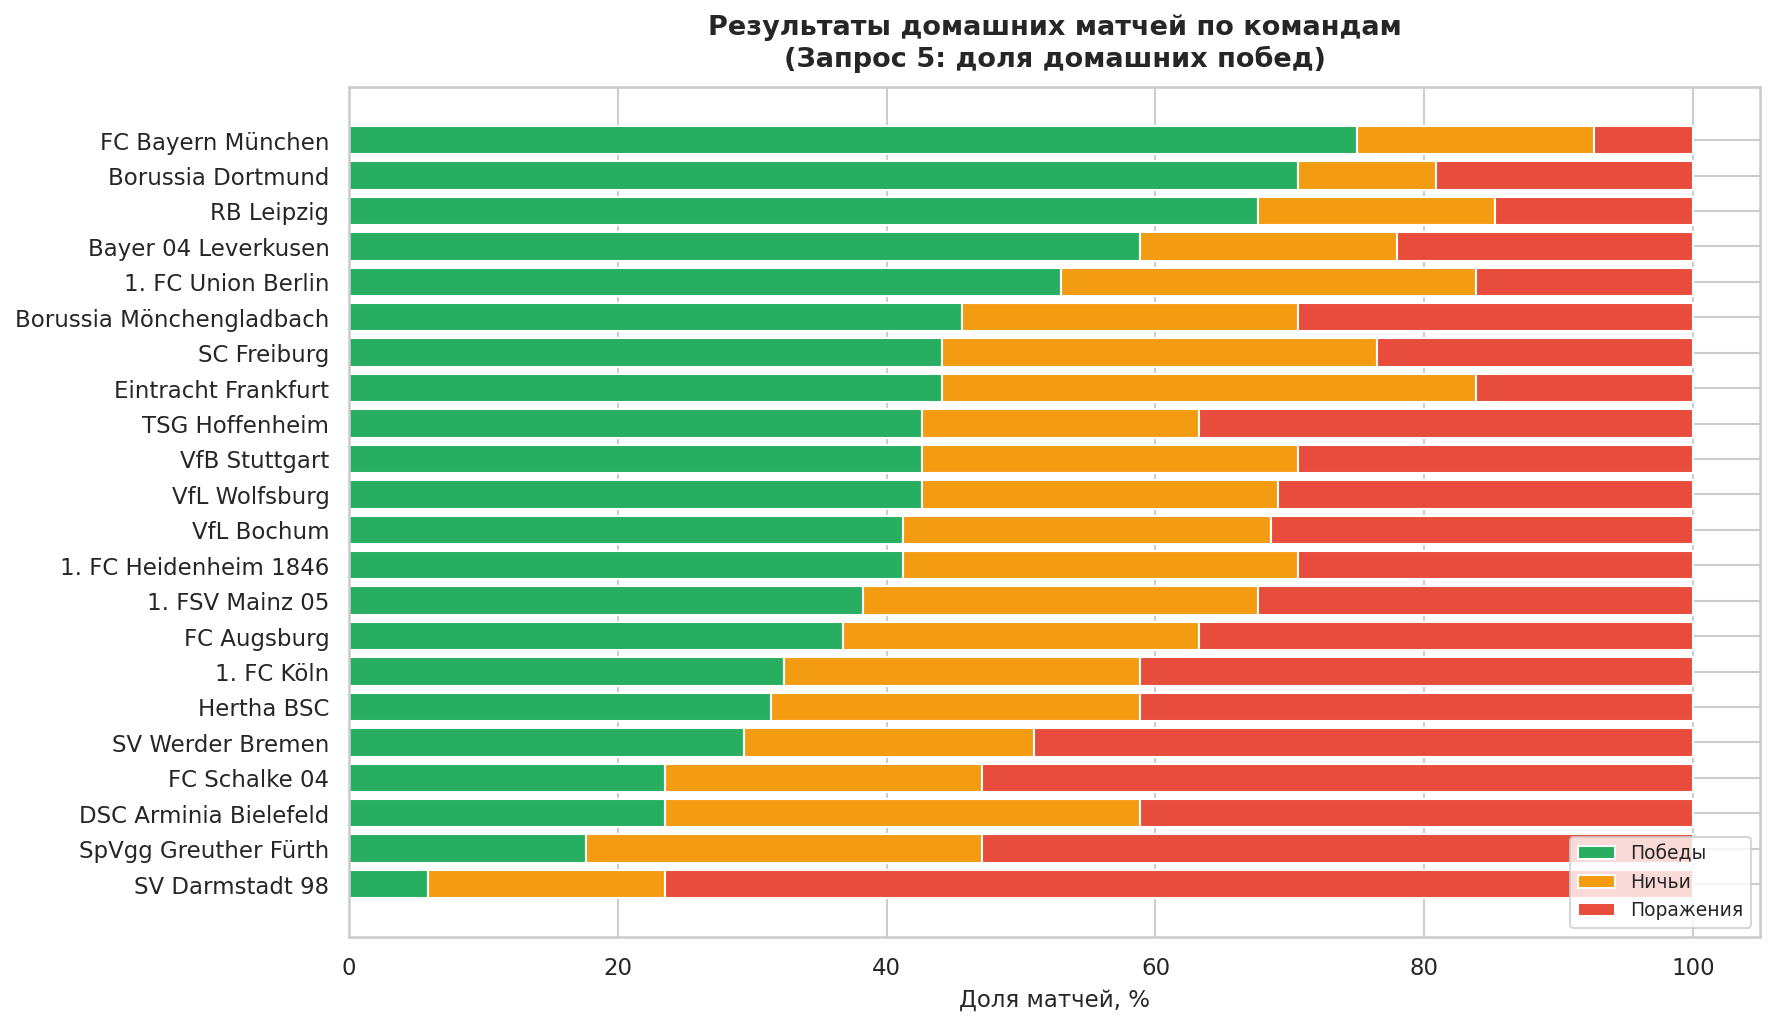
\includegraphics[width=0.95\textwidth]{stage08_viz3_home_wins.png}
  \caption{Домашняя статистика команд (победы / ничьи / поражения дома)}
  \label{fig:viz3}
\end{figure}

% ----------------------------------------------------------
\subsection{График 4. Динамика голов по турам и сезонам}
% ----------------------------------------------------------

\textbf{Тип:} линейный график.\\
\textbf{Данные:} среднее число голов за матч по турам для каждого сезона
(запрос~9).\\
\textbf{Цель:} проследить изменение результативности на протяжении сезонов.

\begin{figure}[H]
  \centering
  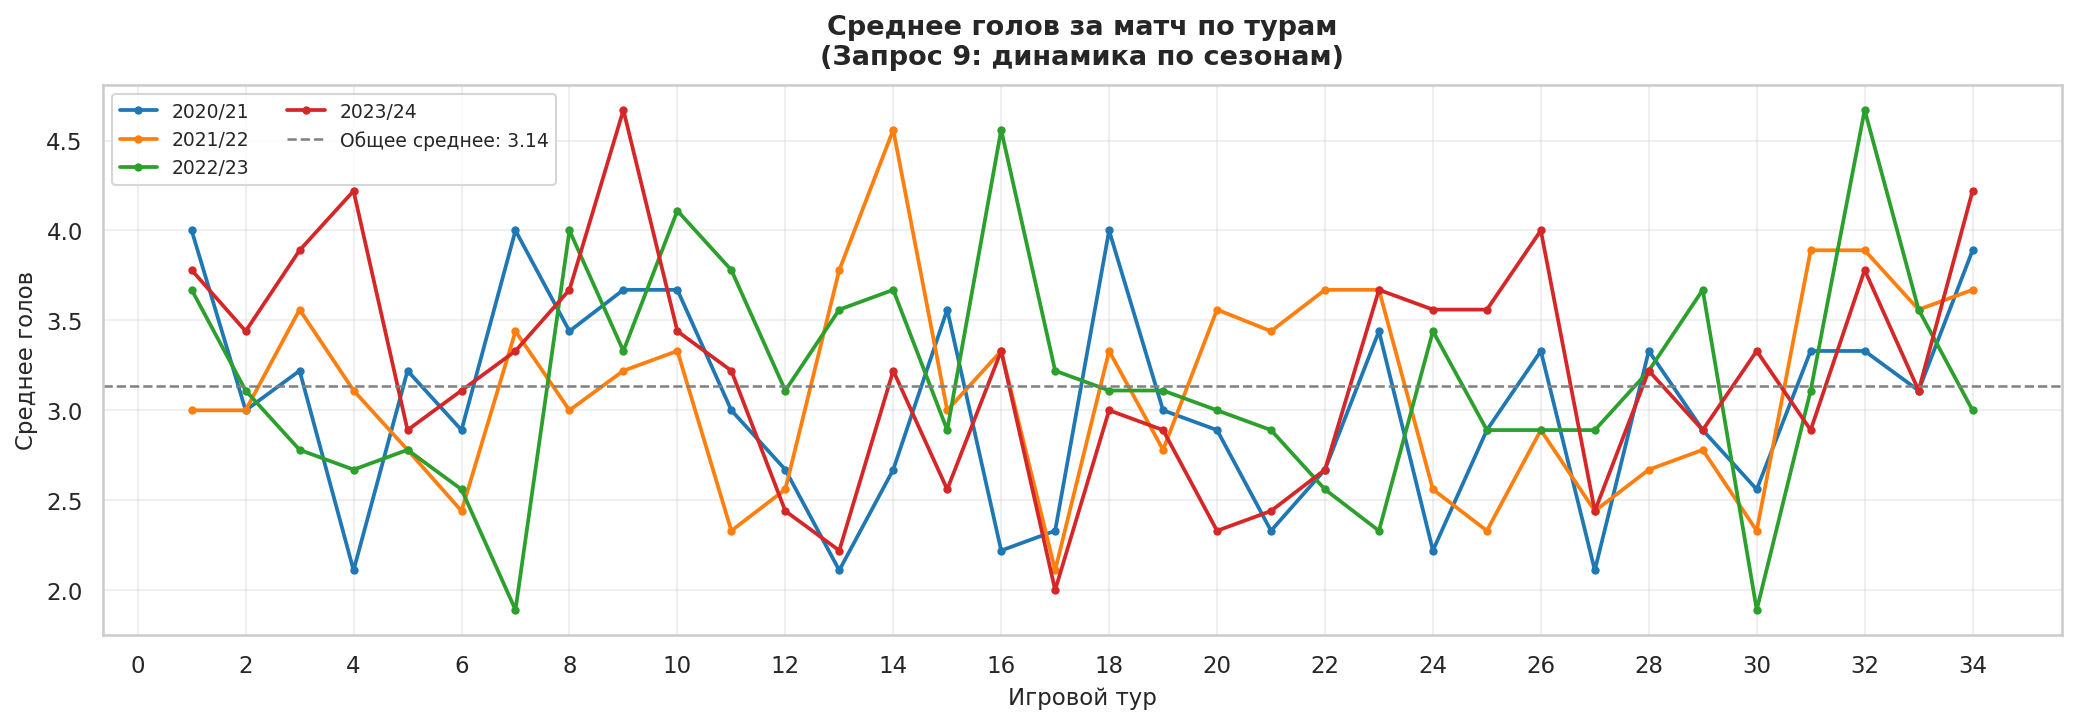
\includegraphics[width=0.95\textwidth]{stage08_viz4_goals_by_matchday.png}
  \caption{Динамика среднего числа голов по турам и сезонам}
  \label{fig:viz4}
\end{figure}

% ----------------------------------------------------------
\subsection{График 5. Нагрузка на судей}
% ----------------------------------------------------------

\textbf{Тип:} сгруппированная гистограмма.\\
\textbf{Данные:} число матчей в роли главного судьи и ассистента для наиболее
загруженных арбитров (запрос~7).\\
\textbf{Цель:} показать распределение судейской нагрузки.

\begin{figure}[H]
  \centering
  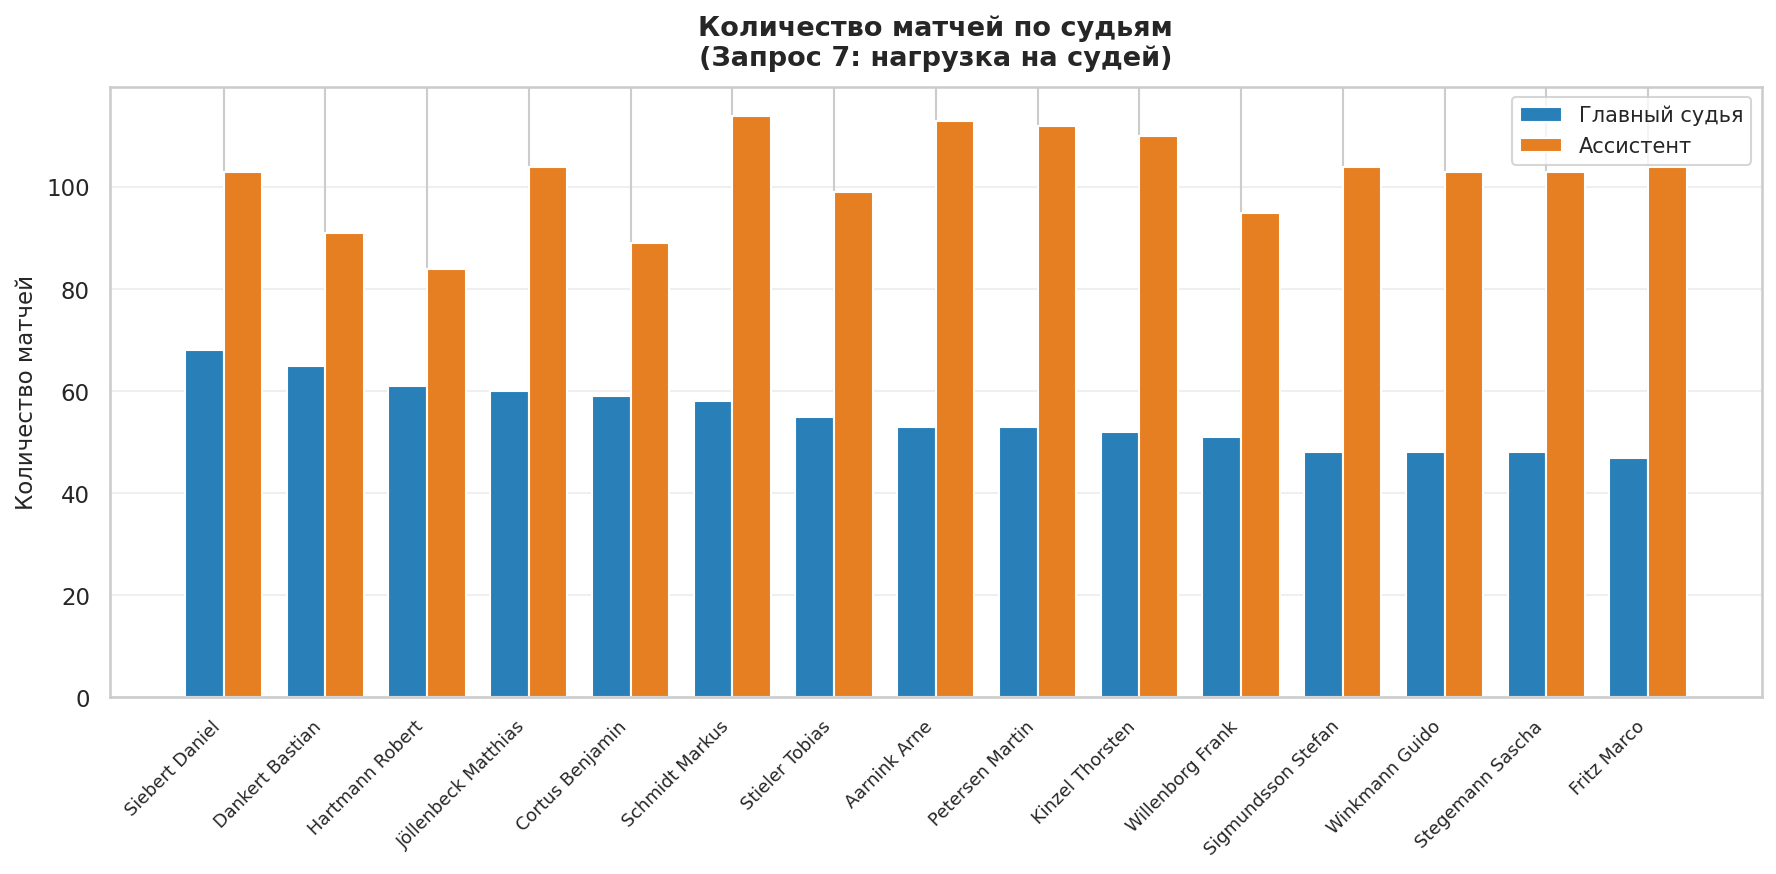
\includegraphics[width=0.95\textwidth]{stage08_viz5_referees.png}
  \caption{Нагрузка на судей Бундеслиги (2020--2023)}
  \label{fig:viz5}
\end{figure}

\section{Заключение}

В ходе выполнения итогового проекта по дисциплине «Хранение и обработка данных»
была спроектирована и реализована реляционная база данных на СУБД PostgreSQL PRO
для предметной области \textbf{«Спортивный турнир»} (Бундеслига, Германия,
сезоны 2020--2023).

\textbf{Результаты работы:}

\begin{itemize}
  \item Разработана структура из 8 взаимосвязанных таблиц с более чем
        3\,000 записей, охватывающих команды, игроков, тренеров, стадионы,
        судей и результаты матчей.
  \item Данные получены из открытого API OpenLigaDB (лицензия CC BY)
        и загружены в базу через скрипты Python.
  \item Реализованы 10 аналитических SQL-запросов, охватывающих расписание
        турнира, турнирные таблицы, статистику по командам, стадионам и судьям,
        а также личные встречи команд.
  \item Подготовлены визуализации на основе данных из БД с помощью библиотек
        \texttt{matplotlib} и \texttt{seaborn}.
\end{itemize}

\textbf{Источник данных:} OpenLigaDB API
(\url{https://www.openligadb.de/}), лицензия CC BY.

\end{document}
